
%(BEGIN_QUESTION)
% Copyright 2006, Tony R. Kuphaldt, released under the Creative Commons Attribution License (v 1.0)
% This means you may do almost anything with this work of mine, so long as you give me proper credit

One simple way to build a ``reference junction compensation'' circuit is to use a bridge with a thermistor (temperature-sensitive resistor) in one arm like this:

$$\includegraphics[width=15.5cm]{i00384x01.eps}$$

As the terminal block warms up and cools down, the resistance of the thermistor will change, altering the balance of the bridge to add the appropriate amount of voltage in series with the meter circuit to cancel out the millivoltage generated by the thermocouple wires connecting with copper wires at the terminal block (the ``reference junction'').

Given the type of thermocouple shown here (type T, with copper and constantan wires), the voltmeter's polarity, the orientation of the battery in the bridge circuit, and the thermistor's location in the bridge circuit, does the thermistor have to have a {\it positive} temperature coefficient (resistance increases as temperature increases) or a {\it negative} temperature coefficient (resistance decreases as temperature increases)?

Hint: begin your solution to the problem by properly identifying the source of the problem itself -- determine the polarity of the reference junction voltage, so you will know which way the bridge's output voltage must be oriented to cancel it out.

\vskip 20pt \vbox{\hrule \hbox{\strut \vrule{} {\bf Suggestions for Socratic discussion} \vrule} \hrule}

\begin{itemize}
\item{} What type of temperature coefficient does an RTD have?
\item{} Suppose the thermistor did not have the right {\it magnitude} of temperature coefficient (i.e. it's ``alpha'' value was wrong).  Would this affect the system's {\it zero}, {\it span}, or both?
\item{} If we must use a thermistor to compensate for the reference junction of a thermocouple, then why use a thermocouple to sense process temperature at all?  Why not just use a thermistor located at the process and be done with it?
\item{} If the thermistor fails open, will it drive the voltmeter upscale or downscale?
\item{} If the thermistor fails shorted, will it drive the voltmeter upscale or downscale?
\end{itemize}

\underbar{file i00384}
%(END_QUESTION)





%(BEGIN_ANSWER)

First, let's determine the polarity of the reference junction's voltage, caused by a joining of constantan (C) and copper (Cu) wires at the lower terminal.  Since we know that copper is the positive wire in a copper-constantan junction, we know that the polarity of the bottom terminal's millivoltage will be positive on the right and negative on the left.  The polarities are shown here both with +/- symbols and also with curved arrows (the arrow tip being positive):

$$\includegraphics[width=15.5cm]{i00384x02.eps}$$

To counter this millivoltage, the bridge circuit's output must be positive on the left and negative on the right:

$$\includegraphics[width=15.5cm]{i00384x03.eps}$$

We know that the warmer the reference junction becomes, the more voltage it will produce.  Thus, the bridge must also produce more countering voltage as the thermistor increases in temperature.  For the left terminal of the bridge circuit to become more positive (and the right terminal, conversely, to become more negative), given a battery orientation that is positive ``up'' and negative ``down,'' the thermistor must {\it decrease} in value.  Therefore, we need a thermistor that has a {\bf negative temperature coefficient}.

\vskip 10pt

Thermocouples still have value as primary sensing elements for temperature because their operating temperature range far exceeds that of thermistors, and they tend to be more rugged as well.


%(END_ANSWER)





%(BEGIN_NOTES)


%INDEX% Measurement, temperature: thermocouple

%(END_NOTES)


